\documentclass[12pt, orivec]{article}
\usepackage{amsmath}
\usepackage{amssymb}    % for \rightsquigarrow
\usepackage{wasysym}	% for frown face
\usepackage[breakable]{tcolorbox}
\usepackage{ulem}
\usepackage{tikz-cd}		% commutative diagrams
\usepackage{tikz}
\usepackage{amsthm}
\usepackage[backend=biber,bibstyle=authoryear,citestyle=authoryearbrack]{biblatex}
\bibliography{../AGI-book}

\newtheorem{theorem}{Theorem}

\ifdefined\chinchin
\usepackage[CJKspace]{xeCJK}
\setCJKmainfont[BoldFont=SimHei,ItalicFont=AR PL KaitiM GB]{SimSun}
\newcommand{\cc}[2]{#1}
\else
\newcommand{\cc}[2]{#2}
\fi

\newcommand{\code}   [1]{{\footnotesize{\ttfamily #1}}}
\newcommand{\tab}{\hspace*{2cm}}
\newcommand{\powerset}{\raisebox{.15\baselineskip}{\Large\ensuremath{\wp}}}
\newcommand*\KB{\vcenter{\hbox{\includegraphics{../KB-symbol.png}}}}
\newcommand*\NewSym[1]{\vcenter{\hbox{\includegraphics[scale=0.5]{#1}}}}

\title{人工智能的知识表述}
\author{甄景贤}

\begin{document}
\setlength{\parindent}{0pt}
\setlength{\parskip}{2.8ex plus0.8ex minus0.8ex}

\maketitle

\section{什么是 model theory?}

举例来说,hyperbolic geometry(双曲几何)可以「实现」为某些 \textbf{模型}: 
\begin{equation}
\vcenter{\hbox{\includegraphics[scale=0.8]{hyperbolic-models.png}}}  \nonumber
\end{equation}
模型不是唯一的,可以有很多种。

在数理逻辑中,\textbf{模型论} 研究的是 syntax / \textbf{theory} 和 \textbf{model} 之间的 \textbf{对偶}。

First-order logic 的 模型 可以用一些 \textbf{集合} 及其 \textbf{元素} 组成。  例如,\\
$\mbox{John} \in \mbox{Male}, \quad \mbox{John, Mary} \in \mbox{Mathematician}$: 
\begin{equation}
\vcenter{\hbox{\includegraphics[scale=0.6]{FOL-model-1.png}}} 
\end{equation}
而 first-order objects(\textbf{个体})之间的 \textbf{关系} 是 domain $D$ 的 Cartesian product $D \times D$ 内的一些 \textbf{子集},例如:
\begin{equation}
\vcenter{\hbox{\includegraphics[scale=0.6]{FOL-model-2.png}}} 
\end{equation}

对计算系的人来说,更熟识的 model 是以下这种 relation graph 或 \textbf{knowledge graph}: 
\begin{equation}
\vcenter{\hbox{\includegraphics[scale=0.6]{FOL-model-3.png}}} 
\end{equation}
但这种 graph 不是数学中最常见的那种,因为它的 \textbf{边} 有 \textbf{labels}。 

以上的 knowledge graph 可以简单地转换成 \textbf{逻辑式子} 的集合:
\footnotesize
\begin{equation}
\begin{array}{l}
	\verb|Loves(John, Mary)| \\
	\verb|Loves(Pete, Mary)| \\
	\verb|Loves(Mary, Pete)| \\
	\verb|Hates(John, Pete)| \\
	\verb|Unhappy(John)|
\end{array}
\label{FOL-model}
\end{equation}
\normalsize
所以说,逻辑 与 graph 基本上是 \textbf{等价} 的。

\begin{tcolorbox}[breakable]
如果 graph 的每条 边 可以包含任意个 顶点,则有 \textbf{hyper-graph}。 换句话说,hypergraph 的每条 边 $\in \powerset(V)$,$V$ 是 顶点集。 也可以说,hypergraph 就是 V 的 \textbf{子集系统} (set system)。  对逻辑来说,这好处是: \uline{关系 之上可以有 关系}。  

Hypergraph 可以一一对应於拓扑学上的 \textbf{simplicial complex},可以研究它的 homology 和 cohomology。 Simplicial complex 也可以和 \textbf{square-free monomial ideals} 一一对应。 Square-free 的意思是 $x_i$ 的指数只可以是 0 或 1。  后者是 \textbf{组合交换代数} (combinatorial commutative algebra) 的研究范围。  暂时我不知道这些关联有没有用,详细可参看 \parencite{Brown2013}, \parencite{Miller2005}。
\end{tcolorbox}

逻辑的 syntactic \textbf{theory} 方面,例如可以有以下这个式子(``失恋则不开心''):
\begin{equation}
\forall x,y. \; \mbox{Loves}(x,y) \wedge \neg \mbox{Loves}(y,x) \rightarrow \mbox{Unhappy}(x)
\end{equation}
这个式子含有 universal quantification,所以不是 model 的一部分。 逻辑上来说,只有 \textbf{ground sentences} (没有变量的式子)的集合才可以组成 model,例如 (\ref{FOL-model}) 。 

所以,logic \textbf{theory} 中的一个式子 可以导致 model 中出现很多 \textbf{新的} 顶点和连接。 这是 model theory 研究的问题。

例如,每一个自然数 $n \in \mathbb{N}$ 都有 它的 successor $S(n)$。 这个函数的存在,导致 model 空间里有一系列 \textbf{无穷} 的顶点:
\begin{equation}
\textbullet \quad \textbullet \quad \textbullet \quad \textbullet \quad \textbullet \quad \textbullet \quad \textbullet \quad \textbullet \quad \textbullet \; .....
\end{equation}
如果加入这条 \textbf{法则}:
\begin{equation}
\forall n \in \mathbb{N}. \quad S(n) \ge n
\end{equation}
则立即产生无穷多个关系:
\begin{equation}
\textbullet \stackrel{\ge}{\longleftarrow} \textbullet \stackrel{\ge}{\longleftarrow} \textbullet \stackrel{\ge}{\longleftarrow} \textbullet \stackrel{\ge}{\longleftarrow} \textbullet \stackrel{\ge}{\longleftarrow} \textbullet \stackrel{\ge}{\longleftarrow} \textbullet \stackrel{\ge}{\longleftarrow} \textbullet \; .....
\end{equation}
虽然,在 \textbf{日常智能} (common-sense intelligence) 中,似乎比较少出现这种无穷的结构,而更多是 ``shallow'' 的结构。 

值得注意的是,经典逻辑人工智能 (classical logic-based AI) 的知识表述 是分拆成 \textbf{rules} 和 \textbf{facts} 两部分。 前者是带有 $\forall$ \textbf{变量} 的式子,后者是 ground sentences。  Rules 储存在 $\KB$ 内,facts 储存在 \textbf{working memory} 内。 前者是一个 \textbf{theory},后者可以看成是一些 \textbf{``partial'' models}。  说 partial 的原因是因为它不代表整个 model。  事实上 model 是非常庞大的东西,不可能储存在物理系统中。  人工智能或大脑只能储存 某种 theories 和部分的 models。  人工智能的关键问题是如何找一种良好的 syntax 结构,令 theory 的学习更快更有效率。 

\section{Distributive representations}

Distributive representation 当然是针对神经网络而言的,因为神经网络是现时最强的机器学习方法(除了我最近开始提倡使用的 \textbf{基因算法})。

Distributive 的意思是: 假设有一个 vector 表示神经网络的输出端有 $n = 10$ 粒神经元:
\begin{equation}
\vec{x} = (x_1, x_2, .... , x_{10})
\end{equation}
用 2 进制,每个 $x_i \in \{ 0, 1 \}$,则 $\vec{x}$ 可以分别表示 10 个 ``\textbf{one-hot}'' 的概念。  但如果用 distributive representation,这 10 个 bits 最多可以表达 $2^n = 1024$ 个不同的状态/概念。  所以 distributiveness 可以非常有效地善用神经元。

假设,「遇见美女过马路」。 这个图像经过譬如 CNN 的处理后,可以得到一个 \textbf{分布式知识表述}:
\begin{equation}
\vcenter{\hbox{\includegraphics[scale=0.7]{NN-activation-patterns.png}}}
\end{equation}
注意那些红点不一定是\textbf{最后}那层的输出。  这是我心目中的图像,比较 general,不是指某个特定的 implementation。  重点是: 「美女过马路」是一个 ``\textbf{neat}'' proposition,但在感知过程中,我们会认得很多细节,例如「裙子、高跟鞋、金发、斑马线、路灯」等。  这些特徵 (features) 构成整个 representation,至少我是这样理解 分布式表述 的。

经典逻辑表述是由 命题 构成的,其实 features 也可以看成是命题,例如「高跟鞋」可以看成是「有一只高跟鞋在这位置」的命题。 逻辑上来说:
\begin{equation}
\boxed{\mbox{neat proposition}} \quad p \Leftrightarrow \bigwedge q_i \quad \boxed{\mbox{distributive features}}
\end{equation}
有时(例如纯文字输入时),知道的只是一个 neat 命题,例如「美女过马路」,并不知道其他细节(例如「金发」),这时仍然可以有分布式表述,但那些特徵会是比较抽象的。

考虑「白猫追黑猫」这个图像:
\begin{equation}
\vcenter{\hbox{\includegraphics[scale=0.7]{white-cat-chase-black-cat.png}}}
\end{equation}
「猫」的概念需要出现 \textbf{两次},但神经网络内对应於「猫」的特徵只有 \textbf{一组}(除非有两个重复的可以表示任何概念的 modules,但很浪费)。 换句话说,现时的 CNN 没有「巡迴 (traverse)」视野域的能力; \uline{它不能辨别和描述物体之间的 }\textbf{\uline{关系}}。  我很难想像一个 ``monolithic'' neural module 怎样可以做到这功能。 似乎必须将命题表述成一连串 概念 的 \textbf{时间序列} (time sequence)。

考虑上节讲过的 逻辑 rule(``失恋则不开心''):
\begin{equation}
\forall x,y. \; x \heartsuit y \wedge \neg y \heartsuit x \rightarrow \frownie{} x
\end{equation}
这个 rule 的 \textbf{前件} (antecedent) 要成立,必须 \uline{两次出现的 $x$ }\textbf{\uline{相等}}\uline{、两次出现的 $y$ }\textbf{\uline{相等}}:
\begin{equation}
\vcenter{\hbox{\includegraphics[scale=0.6]{antecedents-equal.png}}}
\end{equation}
而且,要产生正确的 \textbf{后件} (consequent),需要从前件中将 $x$ \textbf{copy} 过来:
\begin{equation}
\vcenter{\hbox{\includegraphics[scale=0.6]{consequent-copy.png}}}
\end{equation}
\uline{这两个动作(\textbf{compare} 和 \textbf{copy})都是用神经网络 很难做到的}。  但它们是 variable substitution 的本质,也是 谓词逻辑 麻烦之处。 换句话说,很难用一个 monolithic 的 end-to-end 神经网络 一口气完成这两个动作:
\begin{equation}
\vcenter{\hbox{\includegraphics[scale=0.6]{monolithic-NN.png}}}
\end{equation}
事实上,要做到以上功能,似乎必需有一个 \textbf{动态的记忆体},它接收新来的元素时,会对记忆体中其他元素逐一 \textbf{比较},而且具备 \textbf{复制} 功能。  例如我考虑过一个像「迴转木马」的时间序列机制(每个 $\NewSym{distributive-vector.png}$ 代表一支 distributive vector):
\begin{equation}
\vcenter{\hbox{\includegraphics[scale=0.7]{carousel-of-vectors.png}}}
\end{equation}
但仍未解决 compare 和 copy 的问题。 总之,明显地很麻烦。

\section{Graph neural networks}




\section{Genetic algorithm}

这令我想到 \uline{放弃用 neural network 直接处理逻辑,而是用 hybrid 的 神经/逻辑 混合}: 视觉神经用 deep neural network,到高层次转用符号逻辑表述,后者用 genetic algorithm 做学习....

首先有个 logic-based rule engine,它负责 forward-chaining(正向逻辑推导),这完全是经典 AI 范围。 

馀下的问题是要学习那些 rules,这就是 genetic algorithm 做的。 

它的 population 是由个别的 rules 组成,但 winner 并不是单一条 rule,而是一整套 rules(最高分的N个)。 这叫 cooperative co-evolution(COCO)。  

输入和输出是 logic formulas,其实更易处理。 

整个系统仍然是基於 reinforcement learning 的,但不需要直接做 RL,因为那些 rules 其实就是 actions,每一条 rule  的 probabilistic strength 就像 Q-learning 的作用。 


\section{Categorical semantics}

Categorical semantics 是用 category theory 表达的 model theory。  以下内容主要来自 \parencite{Caramello2018} 这本新书的第一章。  更经典的参考书是 \parencite{Goldblatt2006}. 

\begin{equation}
\vcenter{\hbox{\includegraphics[scale=0.7]{logical-categories.png}}}
\end{equation}

\section{Domain theory}

$\lambda$-calculus 和 combinatory logic 都是可以表达任意 \textbf{函数} 的形式。 如果全体函数的 domain 是 $D$,而 由 $D \rightarrow D$ 的函数的个数是 $|D^D|$,则根据集合论的 Cantor's theorem,$|D^D|$ 必定大於 $|D|$,即使 $D$ 是无穷依然成立。 换句话说,$\lambda$-calculus 和 combinatory logic 不可能有 models。  这结论是非常令人不安的。 但这个问题被 Dana Scott 和 C Strachey 在 1971 年解决了,开创了 \textbf{domain theory}。

以下内容主要来自 \parencite{Vickers1989},是一本很易懂的书,还有更新的和更详尽的 \parencite{Goubault-Larrecq2013}.


\section{Group theory}

\printbibliography

\end{document}